\section*{Ergbnisse}
%\begin{frame}
%    \frametitle{Conclusion}
%    \begin{itemize}    
%        \item Performance im Vergleich zu TD3 und A2C
%        \item Vor- und Nachteile von SAC
%    \end{itemize}
%\end{frame}




\begin{frame}{Ziel der Experimente}
        \begin{itemize}
            \item Stabilität und Sample Komplexität im Vergleich zu anderen Algorithmen
            \begin{itemize}
                \item kontinuierliche Aufgaben
                \item verschiedene Schwierigkeitgrade
            \end{itemize}  
            \item OpenAI gym und rllab
        \end{itemize}
\end{frame}

\begin{frame}{Vergleich zu anderen Algorithmen}
    \begin{itemize}
        \item SAC
        \begin{itemize}
            \item mean action
            \item feste und variable Temperatur
        \end{itemize} 
        \item PPO
        \item DDPG
        \item TD3
        \item SQL mit zwei Q Funktionen
        \begin{itemize}
            \item evaluated with exploration noise
        
        \end{itemize}
        \item 5 Instanzen mit einer Evaluation alle 1000 Schritte
        \item Total average return shown in the following
        \item schattierter Verlauf sind alle fünf Durchläufe
        
    \end{itemize}
        
\end{frame}

\begin{frame}
    \frametitle{Ergebnisse}
    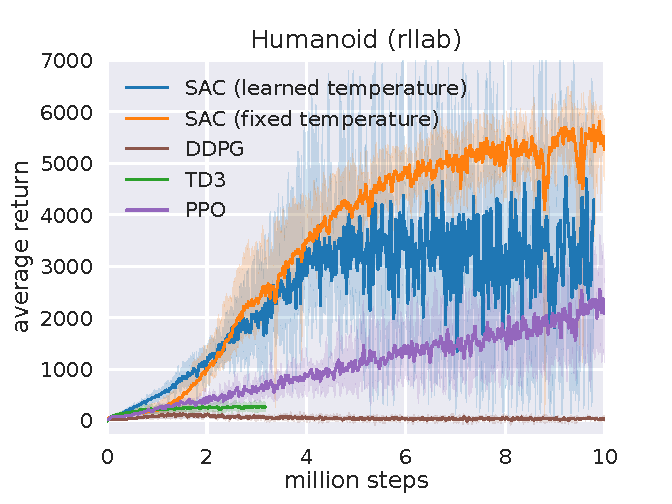
\includegraphics[scale=0.8]{figures/humanoid-rllab.pdf}
\end{frame}
\note{
    DDPG = Deep Deterministic Policy Gradiend 
    TD3 =  Twin deep Deterministic gradiend
}
\begin{frame}
    \frametitle{Ergebnisse}
    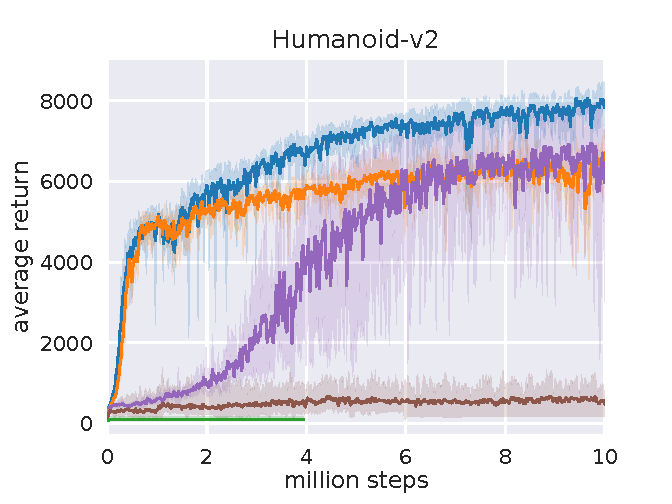
\includegraphics[scale=0.8]{figures/humanoid-gym.pdf}
\end{frame}
\begin{frame}
    \frametitle{Ergebnisse}
    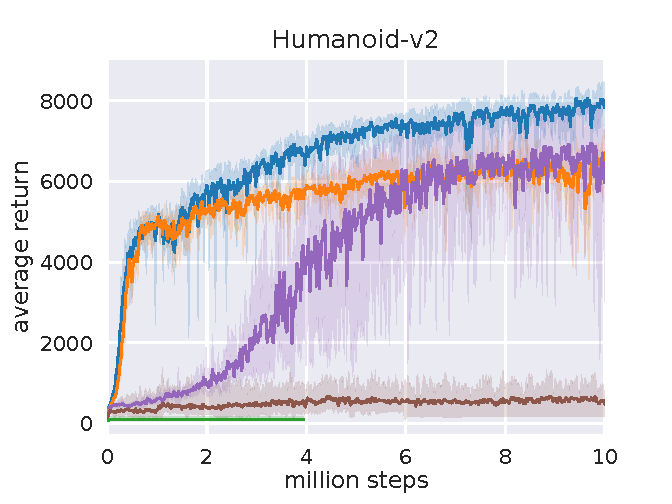
\includegraphics[scale=0.8]{figures/humanoid-gym-backup-2.pdf}
\end{frame}


\begin{frame}
    \frametitle{Ergebnisse}
    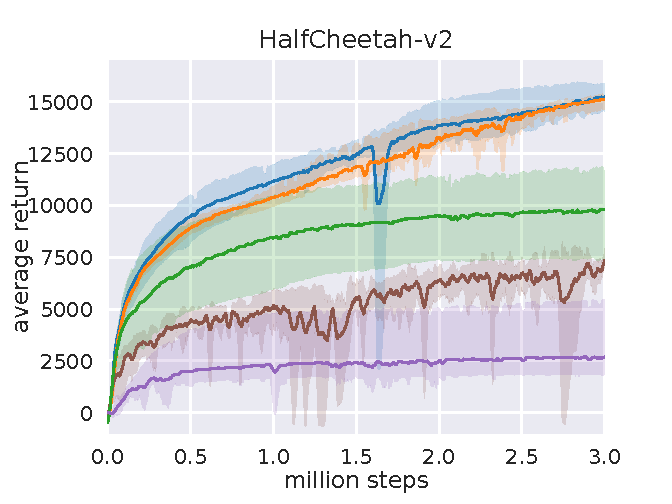
\includegraphics[scale=0.8]{figures/half-cheetah.pdf}
\end{frame}
\begin{frame}
    \frametitle{Ergebnisse}
    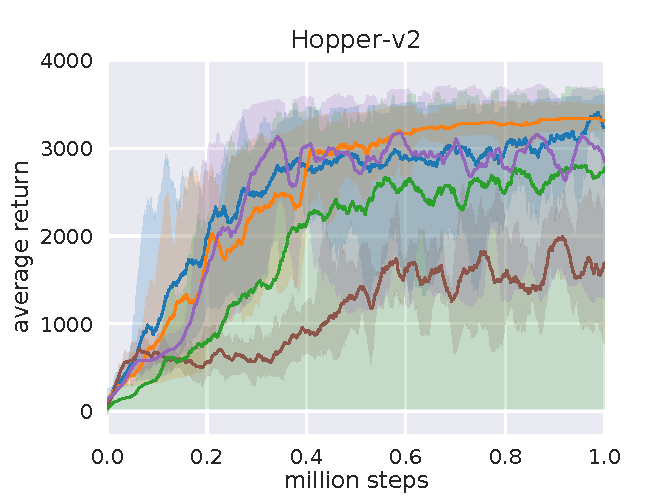
\includegraphics[scale=0.8]{figures/hopper.pdf}
\end{frame}
\begin{frame}
    \frametitle{Ergebnisse}
    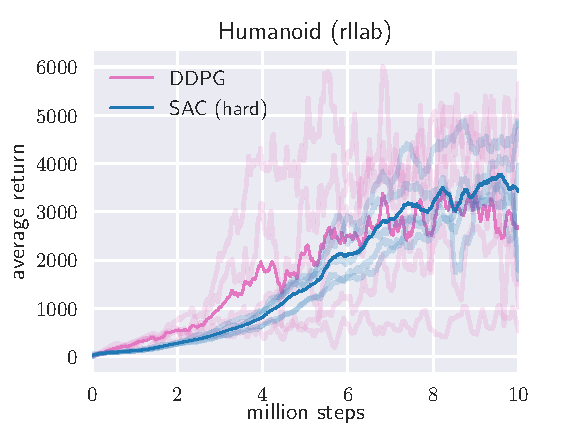
\includegraphics[scale=0.8]{figures/seeds-humanoid.pdf}
\end{frame}
\begin{frame}
    \frametitle{Ergebnisse}
    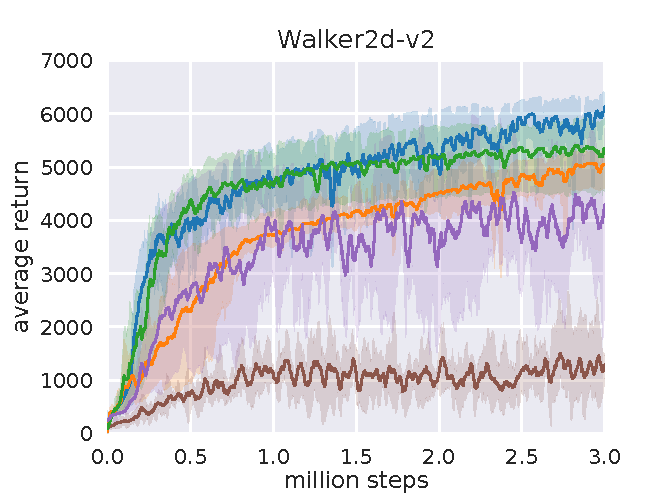
\includegraphics[scale=0.8]{figures/walker.pdf}
\end{frame}

\begin{frame}
    \frametitle{Ergebnisse}
    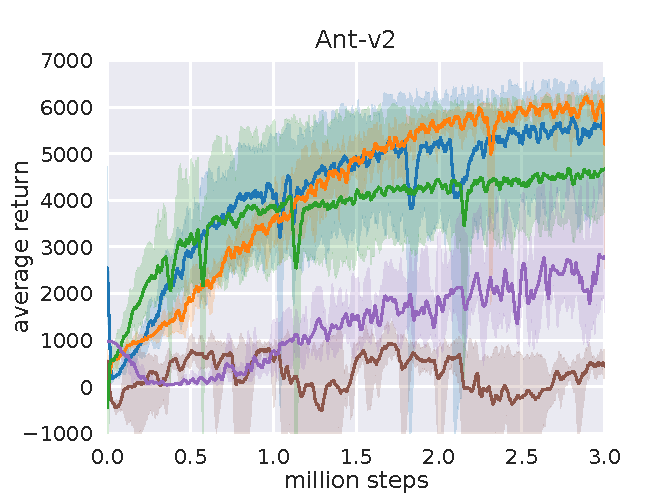
\includegraphics[scale=0.8]{figures/ant.pdf}
\end{frame}


\begin{frame}{Zusammenfassung}
        \begin{itemize}
            \item soft actor critic vorgestellt
            \begin{itemize}
                \item off policy
                \item Entropiemaximierung verbessert Stabilität
                \item Besser als state of the art Algorithmen 
            \end{itemize} 
        \end{itemize}
\end{frame}

